\documentclass[10pt]{beamer}
\usetheme{Singapore}
%\usetheme{CambridgeUS}
\usepackage{mathpazo}
\usepackage[OT1]{fontenc}


\usepackage{array} % needed for \arraybackslash
\usepackage{adjustbox} % for \adjincludegraphics
\usepackage{graphicx}
\usepackage{epstopdf}
\usepackage{xmpmulti}
\usepackage{subcaption}
\usepackage{nicefrac}
\captionsetup{compatibility=false}

% AMS Math, Symbol and Theorem packages
\usepackage{amssymb}
\usepackage{amsthm}
\usepackage{amsmath}
%\usepackage{enumitem}
%\usepackage{empheq}
\usepackage{bigstrut}

% Theorem declarations
\theoremstyle{plain}
% new commands
%\newcommand{\Nor}{{\cal N}}
%\newcommand{\half}{\frac{1}{2}}
%\newcommand{\quart}{\frac{1}{4}}
%\newcommand{\ben}{\begin{enumerate}}
%\newcommand{\een}{\end{enumerate}}
%\newcommand{\beq}{\begin{equation}}
%\newcommand{\eeq}{\end{equation}}
%\newcommand{\bit}{\begin{itemize}}
%\newcommand{\eit}{\end{itemize}}
%\newcommand{\bde}{\begin{description}}
%\newcommand{\ede}{\end{description}}



% \mathcolor{<color>}{<stuff>}
\makeatletter
\def\mathcolor#1#{\@mathcolor{#1}}
\def\@mathcolor#1#2#3{%
  \protect\leavevmode
  \begingroup
    \color#1{#2}#3%
  \endgroup
}
\makeatother


%%%%%%
\usepackage{color}
\definecolor{DarkBlue}{rgb}{0.1,0.1,0.5}
\definecolor{Red}{rgb}{0.9,0.0,0.1}
\definecolor{Navy}{rgb}{0.00,0.00,0.30}
\definecolor{Yellow}{rgb}{1.00,1.00,0.00}
\definecolor{Gold}{rgb}{1.00,0.84,0.00}
\definecolor{Lightgoldenrod}{rgb}{0.93,0.87,0.51}
\definecolor{Goldenrod}{rgb}{0.85,0.65,0.13}
\definecolor{Black2}{rgb}{0.00,0.00,0.00}
\definecolor{orange}{rgb}{0.85,0.65,0.13}
\definecolor{SkyBlue}{rgb}{0.941176,0.972549,1.}
\definecolor{MyLightMagenta}{cmyk}{0.1,0.8,0,0.1}
%%%%%
\usepackage{xcolor}
%% \highlight[<colour>]{<stuff>}
\newcommand{\highlight}[2][yellow]{\mathchoice%
  {\colorbox{#1}{$\displaystyle#2$}}%
  {\colorbox{#1}{$\textstyle#2$}}%
  {\colorbox{#1}{$\scriptstyle#2$}}%
  {\colorbox{#1}{$\scriptscriptstyle#2$}}}%

%%% see documentation for a0poster class for the size options here
%% These are helpful for creating huge fonts on a slide. More useful for making posters. 

\let\Textsize\normalsize
\def\Head#1{\noindent\hbox to \hsize{\hfil{\LARGE\color{DarkBlue} #1}}\bigskip}
\def\LHead#1{\noindent{\LARGE\color{DarkBlue} #1}\smallskip}
%%\def\Subhead#1{\noindent{\large\color{DarkBlue} #1}}
%%\def\Title#1{\noindent{\VeryHuge\color{Red} #1}}
\def\Subhead#1{\noindent{\large\color{Black2} #1}}
\def\Title#1{\begin{center} \LARGE\bf{\color{Black2} #1}\end{center}}
\def\heading#1{\begin{center} \Large\bf{\color{DarkBlue} #1}
\end{center} } %\vspace{1ex minus 1ex}

%% We don't need abstract in slides
%\def\abstract{\begin{flushleft} \Large\bf{\color{DarkBlue} }
%\end{flushleft} } %\vspace{1ex minus 1ex}

\usepackage{array} % needed for \arraybackslash
\newcolumntype{L}[1]{>{\raggedright\let\newline\\\arraybackslash\hspace{0pt}}m{#1}}
\newcolumntype{C}[1]{>{\centering\let\newline\\\arraybackslash\hspace{0pt}}m{#1}}
\newcolumntype{R}[1]{>{\raggedleft\let\newline\\\arraybackslash\hspace{0pt}}m{#1}}

% To add some paragraph space between lines.
% This also tells LaTeX to preferably break a page on one of these gaps
% if there is a needed pagebreak nearby.
\newcommand{\blankline}{\quad\pagebreak[3]}
\newcommand{\halfblankline}{\quad\vspace{-0.5\baselineskip}\pagebreak[3]}

%
% Math commands by Thomas Minka 
%
% Revised by Jyotishka Datta & Brandon Willard
% Acknowledgement: JD received this from Prof. Alan Qi.
%


%% Special shortcuts for us
\def\Polya{P{\'o}lya}
\def\CS{Cauchy-Schl\"omilch}
\def\PG{P{\'o}lya-Gamma}

%\setlength{\textfloatsep}{10pt plus 1.0pt minus 2.0pt}
%\setlength{\floatsep}{12.0pt plus 2.0pt minus 5.0pt}
%\setlength{\intextsep}{12.0pt plus 2.0pt minus 5.0pt}
%\setlength{\belowcaptionskip}{-2pt}

%\def\distrib{\mathrel{\ooalign{%
%  \raisebox{0.75\height}{{\small{ind}}}\cr\hidewidth$\sim$\hidewidth\cr}}}
%  
\newcommand{\var}{{\rm var}}
\newcommand{\Tr}{^{\rm T}}
\newcommand{\rmlog}{\rm log}
\newcommand{\vtrans}[2]{{#1}^{(#2)}}
\newcommand{\kron}{\otimes}
\newcommand{\schur}[2]{({#1} | {#2})}
\newcommand{\schurdet}[2]{\left| ({#1} | {#2}) \right|}
\newcommand{\had}{\circ}
\newcommand{\diag}{{\rm diag}}
\newcommand{\invdiag}{\diag^{-1}}
\newcommand{\rank}{{\rm rank}}
% careful: ``null'' is already a latex command
\newcommand{\nullsp}{{\rm null}}
\newcommand{\tr}{{\rm tr}}
\renewcommand{\vec}{{\rm vec}}
\newcommand{\vech}{{\rm vech}}
\renewcommand{\det}[1]{\left| #1 \right|}
\newcommand{\pdet}[1]{\left| #1 \right|_{+}}
\newcommand{\pinv}[1]{#1^{+}}
\newcommand{\erf}{{\rm erf}}
\newcommand{\hypergeom}[2]{{}_{#1}F_{#2}}

% boldface characters
\renewcommand{\a}{{\bf a}}
\renewcommand{\b}{{\bf b}}
\renewcommand{\c}{{\bf c}}
\renewcommand{\d}{{\rm d}}  % for derivatives
\newcommand{\e}{{\rm e}} % for exponentials
\newcommand{\f}{{\bf f}}
\newcommand{\g}{{\bf g}}
\newcommand{\h}{{\bf h}}
%\newcommand{\k}{{\bf k}}
% in Latex2e this must be renewcommand
\renewcommand{\k}{{\bf k}}
\newcommand{\m}{{\bf m}}
\newcommand{\n}{{\bf n}}
%\renewcommand{\o}{{\bf o}}
\newcommand{\p}{{\bf p}}
%\newcommand{\q}{{\bf q}}
\renewcommand{\r}{{\bf r}}
\newcommand{\s}{{\bf s}}
\renewcommand{\t}{{\bf t}}
\renewcommand{\u}{{\bf u}}
\renewcommand{\v}{{\bf v}}
\newcommand{\w}{{\bf w}}
%\newcommand{\x}{{\bf x}}
\newcommand{\y}{{\bf y}}
%\newcommand{\z}{{\bf z}}
\newcommand{\A}{{\bf A}}
\newcommand{\B}{{\bf B}}
\newcommand{\C}{{\bf C}}
\newcommand{\D}{{\bf D}}
\newcommand{\E}{{\bf E}}
\newcommand{\F}{{\bf F}}
%\newcommand{\G}{{\bf G}}
\renewcommand{\H}{{\bf H}}
\newcommand{\I}{{\bf I}}
\newcommand{\J}{{\bf J}}
\newcommand{\K}{{\bf K}}
\renewcommand{\L}{{\bf L}}
\newcommand{\M}{{\bf M}}
%\newcommand{\N}{{\bf N}}
\renewcommand{\O}{{\bf O}}
\renewcommand{\P}{{\bf P}}
\newcommand{\Q}{{\bf Q}}
\newcommand{\R}{{\bf R}}
%\renewcommand{\S}{{\bf S}}
\newcommand{\T}{{\rm T}}
%\newcommand{\U}{{\bf U}}
\newcommand{\V}{{\bf V}}
\newcommand{\W}{{\bf W}}
\newcommand{\X}{{\bf X}}
\newcommand{\Y}{{\bf Y}}
\newcommand{\Z}{{\bf Z}}

% this is for latex 2.09
% unfortunately, the result is slanted - use Latex2e instead
%\newcommand{\bfLambda}{\mbox{\boldmath$\Lambda$}}
% this is for Latex2e
\newcommand{\bfLambda}{\boldsymbol{\Lambda}}

% Yuan Qi's boldsymbol
\newcommand{\bsigma}{\boldsymbol{\sigma}}
\newcommand{\balpha}{\boldsymbol{\alpha}}
\newcommand{\bpsi}{\boldsymbol{\psi}}
\newcommand{\bphi}{\boldsymbol{\phi}}
\newcommand{\bbeta}{\boldsymbol{\beta}}
%\newcommand{\Beta}{\boldsymbol{\eta}}
\newcommand{\btau}{\boldsymbol{\tau}}
\newcommand{\bvarphi}{\boldsymbol{\varphi}}
\newcommand{\bzeta}{\boldsymbol{\zeta}}
\newcommand{\bnabla}{\boldsymbol{\nabla}}
\newcommand{\blambda}{\boldsymbol{\lambda}}
\newcommand{\bLambda}{\mathbf{\Lambda}}

\newcommand{\btheta}{\boldsymbol{\theta}}
\newcommand{\bpi}{\boldsymbol{\pi}}
\newcommand{\bPi}{\boldsymbol{\Pi}}
\newcommand{\bxi}{\boldsymbol{\xi}}
\newcommand{\bSigma}{\boldsymbol{\Sigma}}

\newcommand{\bgamma}{\mathbf{\gamma}}
\newcommand{\bGamma}{\mathbf{\Gamma}}

\newcommand{\bmu}{\boldsymbol{\mu}}
\newcommand{\bnu}{\boldsymbol{\nu}}
\newcommand{\bPsi}{\mathbf{\Psi}}
\newcommand{\bepsilon}{\boldsymbol{\epsilon}}
\newcommand{\bOmega}{\boldsymbol{\Omega}}

\newcommand{\1}{{\bf 1}}
\newcommand{\0}{{\bf 0}}

%\newcommand{\comment}[1]{}

\newcommand{\bs}{\backslash}
\newcommand{\ben}{\begin{enumerate}}
\newcommand{\een}{\end{enumerate}}
\newcommand{\beq}{\begin{equation}}
\newcommand{\eeq}{\end{equation}}
\newcommand{\bde}{\begin{description}}
\newcommand{\ede}{\end{description}}

\newcommand{\notS}{{\backslash S}}
\newcommand{\nots}{{\backslash s}}
\newcommand{\noti}{{\backslash i}}
\newcommand{\notj}{{\backslash j}}
\newcommand{\nott}{\backslash t}
\newcommand{\notone}{{\backslash 1}}
\newcommand{\nottp}{\backslash t+1}
% \newcommand{\notz}{\backslash z}

\newcommand{\notk}{{^{\backslash k}}}
%\newcommand{\noti}{{^{\backslash i}}}
\newcommand{\notij}{{^{\backslash i,j}}}
\newcommand{\notg}{{^{\backslash g}}}
\newcommand{\wnoti}{{_{\w}^{\backslash i}}}
\newcommand{\wnotg}{{_{\w}^{\backslash g}}}
\newcommand{\vnotij}{{_{\v}^{\backslash i,j}}}
\newcommand{\vnotg}{{_{\v}^{\backslash g}}}
\newcommand{\half}{\frac{1}{2}}
\newcommand{\quart}{\frac{1}{4}}
\newcommand{\msgb}{m_{t \leftarrow t+1}}
\newcommand{\msgf}{m_{t \rightarrow t+1}}
\newcommand{\msgfp}{m_{t-1 \rightarrow t}}

\newcommand{\proj}[1]{{\rm proj}\negmedspace\left[#1\right]}
\newcommand{\argmin}{\operatornamewithlimits{argmin}}
\newcommand{\argmax}{\operatornamewithlimits{argmax}}

\newcommand{\dif}{\mathrm{d}}
\newcommand{\abs}[1]{\lvert#1\rvert}
\newcommand{\norm}[1]{\lVert#1\rVert}
\newcommand{\vectornorm}[1]{\left|\left|#1\right|\right|}

\newcommand{\Nor}{\mathcal{N}}
\newcommand{\NormRV}{\mathcal{N}}
\newcommand{\InvGaussRV}{\mathcal{IG}}
\newcommand{\CauchyRV}{\mathcal{C}}
\newcommand{\GammaRV}{\mathcal{G}}
\newcommand{\UnifRV}{\mathcal{U}}

\newcommand{\bx}{{\bf x}}
\newcommand{\ba}{{\bf a}}
\newcommand{\bb}{{\bf b}}
\newcommand{\bc}{{\bf c}}
\newcommand{\bd}{{\bf d}}
\newcommand{\bX}{{\bf X}}
\newcommand{\by}{{\bf y}}
\newcommand{\dd}[2]{\frac{\partial #1}{\partial #2}}
\newcommand{\lhat}[1][i]{\hat\lambda_{#1}^{-1(g)}}
\newcommand{\what}[1][j]{\hat\omega_{#1}^{-1(g)}}
\newcommand{\bone}{{\bf 1}}
\newcommand{\Li}{\hat\Lambda^{-1(g)}}
\newcommand{\Oi}{\hat\Omega^{-1(g)}}
\newcommand{\iid}{\stackrel{\mathrm{iid}}{\sim}}
\newcommand{\id}{\stackrel{\mathrm{ind}}{\sim}}
\newcommand{\iidp}{\stackrel{\mathrm{P}}{=}}
\newcommand{\iidd}{\stackrel{\mathrm{D}}{=}}
\newcommand{\defeq}{\operatorname{:=}}

% the last {} is a hack for double subscript errors
\newcommand{\estHsp}{\ensuremath{{\hat{\theta}}_{HS+}}{}}
\newcommand{\estHs}{\ensuremath{{\hat{\theta}}_{HS}}{}}
\newcommand{\estJs}{\ensuremath{{\hat{\theta}}_{JS}}{}}
\newcommand{\MSE}{\mathrm{MSE}}

%% INTEGRALS 

\newcommand{\intreal}{\int_{-\infty}^{\infty}}
\newcommand{\intpos}{\int_{0}^{\infty}}
\newcommand{\intunit}{\int_{0}^{1}}


%\newtheorem{theorem}{THEOREM}
%\numberwithin{theorem}{section}
%\newtheorem{Proof}{PROOF}
%\newtheorem{Def}{DEFINITION}
%\numberwithin{Def}{section}
%\newtheorem{remark}{REMARK}
%\numberwithin{remark}{section}
%\newtheorem{Qes}{Question}
%\newtheorem{proposition}{PROPOSITION}
%\numberwithin{proposition}{section}
%\newtheorem{lemma}{LEMMA}
%\numberwithin{lemma}{section}
%\newtheorem{Cor}{COROLLARY}
%\numberwithin{Cor}{section}
%\newtheorem{Exa}{Example}
%\newtheorem{Eq}{Equation}
%\newtheorem{assn}{ASSUMPTION}
%\newtheorem{result}[theorem]{Result}
%\newtheorem{result}[theorem]{RESULT}

%\newtheoremstyle{slplain}% name
%  {1\baselineskip\@plus.2\baselineskip\@minus.2\baselineskip}% Space above
%  {.5\baselineskip\@plus.2\baselineskip\@minus.2\baselineskip}% Space below
%  {\slshape}% Body font
%  {}%Indent amount (empty = no indent, \parindent = para indent)
%  {\bfseries}%  Thm head font
%  {.}%       Punctuation after thm head
%  { }%      Space after thm head: " " = normal interword space;
%        %       \newline = linebreak
%  {}%       Thm head spec
%
%
%\theoremstyle{slplain}

\newtheorem{theorem}{Theorem}
\newtheorem{acknowledgement}[theorem]{Acknowledgement}
%\newtheorem{algorithm}[theorem]{Algorithm}
\newtheorem{axiom}[theorem]{Axiom}
\newtheorem{case}[theorem]{Case}
\newtheorem{claim}[theorem]{Claim}
\newtheorem{conclusion}[theorem]{Conclusion}
\newtheorem{condition}[theorem]{Condition}
\newtheorem{conjecture}[theorem]{Conjecture}
\newtheorem{corollary}[theorem]{Corollary}
\newtheorem{criterion}[theorem]{Criterion}
\newtheorem{definition}[theorem]{Definition}
\newtheorem{example}[theorem]{Example}
\newtheorem{exercise}[theorem]{Exercise}
\newtheorem{lemma}[theorem]{Lemma}
\newtheorem{notation}[theorem]{Notation}
\newtheorem{problem}[theorem]{Problem}
\newtheorem{proposition}[theorem]{Proposition}
\newtheorem{remark}[theorem]{Remark}
\newtheorem{solution}[theorem]{Solution}
\newtheorem{summary}[theorem]{Summary}

\usepackage{booktabs,array}
\def\Midrule{\midrule[\heavyrulewidth]}
\newcount\rowc

%
%\makeatletter
%\def\ttabular{%
%\hbox\bgroup
%\let\\\cr
%\def\rulea{\ifnum\rowc=\@ne \hrule height 1.0pt \fi}
%\def\ruleb{
%\ifnum\rowc=1\hrule height 1.0pt  \else
%%\ifnum\rowc=3\hrule height 0.0pt%\heavyrulewidth 
%\ifnum\rowc= 3  \hrule height 0.5pt \else%\heavyrulewidth 
%\ifnum\rowc= 5  \hrule height 0.5pt \else%\heavyrulewidth 
%\ifnum\rowc= 7  \hrule height 0.5pt \else%\heavyrulewidth 
%\ifnum\rowc= 9  \hrule height 0.5pt \else%\heavyrulewidth 
%\ifnum\rowc= 11  \hrule height 0.5pt %\heavyrulewidth 
  %\else \hrule height 0pt%\lightrulewidth
%\fi\fi\fi\fi\fi\fi}
%\valign\bgroup
%\global\rowc\@ne
%\rulea
%\hbox to 7em{\strut \hfill##\hfill}%
%\ruleb
%&&%
%\global\advance\rowc\@ne
%\hbox to 7em{\strut\hfill##\hfill}%
%\ruleb
%\cr}
%\def\endttabular{%
%\crcr\egroup\egroup}
%

%\graphicspath{{./art/}}
%\pagenumbering{arabic}
\usepackage{natbib} %citep and citet
%\renewcommand{\bibsection}{\subsubsection*{\bibname}}
%\bibpunct[:]{(}{)}{;}{a}{}{,}
\def\sql{$\sqrt{\text{Lasso }}$}
\def\sqdl{$\sqrt{\text{DL }}$}
\usepackage{bibentry}
%\nobibliography*

\title[Adapting to Sparsity and Heavy Tailed Data]{Adapting to Sparsity and Heavy Tailed Data}
\author{Mohamed Abdelkader Abba \thanks{Under the supervision of Dr. J. Datta }}
\institute[UArkansas]{University of Arkansas, Department of Mathematical Sciences}
\date{July 2, 2018}

 %%logo of my university
% \titlegraphic{\includegraphics[width=3.75cm,height=1.2cm]{plots/default/uarklogo}}

% -- Many ways of creatin an outline -- %%
\AtBeginSection[]
{
  \begin{frame}<beamer>
    \frametitle{Outline}
    \tableofcontents[currentsection]
    \pagenumbering{gobble}
  \end{frame}
}

%\AtBeginSection[]{
    %\begin{frame}[noframenumbering, plain]
        %\frametitle{Outline for Today's talk}
        %\tableofcontents[currentsection]
    %\end{frame}
%}

\setbeamertemplate{navigation symbols}{}
\setbeamertemplate{footline}[frame number]
%\renewcommand{\inserttotalframenumber}{60}

\begin{document}


\begin{frame}
\titlepage
\end{frame}

\tableofcontents

\section{Motivation}

\begin{frame}
\frametitle{Sparsity}
Many modern applications of statistical inference involve wide data sets, where the number of features $p \gg n$. 

Examples include, gene expression data, finance, astronomy...

The most popular of these problems are: 
\begin{itemize}
	\item sparse normal means: $(Y_i \mid \beta_i)  \id \Nor (\beta_i,1), i = 1, \dots, n$;
	\item sparse linear regression: $\Y = \X \bbeta + \bepsilon$, $\bepsilon \sim \Nor(\0, \I)$, 
\end{itemize}
where $\bbeta$ is a `nearly black object', that is, 
\[
\bbeta \in l_0 [ p_n] \equiv \{ \bbeta : \# ( \beta_i \neq 0 ) \leq p_n \}
\]

\end{frame}

\begin{frame}
\frametitle{Penalized Regression}
\bit
\item Rich variety of methodologies for high-dimensional inference based on regularization which implicitly or explicitly penalizes model complexity. 

\item This amounts to controlling the bias-variance trade-off and are particularly useful for sparse learning, when the number of variables ($p$) exceed the number of observations ($n$). 

\item In the context of linear regression $Y = X \bbeta + \bepsilon$, a regularized estimate of $\bbeta$ is obtained by minimizing the penalized likelihood:
\eit 

\begin{align}
\hat{\bbeta}_{\lambda^*}^{\text{pen}} & = \argmin_{\bbeta \in \Re^p} \{ \vectornorm{Y - X\bbeta}^2 + \lambda^* \Omega(\bbeta) \}, \label{eq:penalize} \\
  \text{where, } & \Omega(\bbeta) = \sum_{j=1}^{p} \omega(\beta_j) \text{ is a separable penalty}
\end{align}


\end{frame}

\begin{frame}
\frametitle{Lasso}
The gold standard for regularized methods, simultaneously performs estimation and model selection. Lasso constrains the $\ell_1$ norm of the parameter vector:
\beq
\hat{\bbeta}_{\lambda^*}^{\text{lasso}} = \argmin_{\bbeta \in \Re^p} \{ \vectornorm{Y - X\bbeta}^2 + \lambda^* \norm{\bbeta}_1 \} \label{eq:lasso}
\eeq 
\blankline
Lasso enjoys both:
\begin{itemize}
	\item computational efficiency, due to the LARS \cite{efron_least_2004};
	\item theoretical optimality properties in recovering the true $\bbeta_0$ \citet{buhlmann2011statistics}.
\end{itemize}
\end{frame}

\begin{frame}
\frametitle{\sql}
Lasso presents two major drawbacks:
\begin{itemize}
	\item dependence on knowledge / estimation of $\bsigma$, this is particularly problematic when $p \gg n$;
	\item estimates are not scale invariant: $\hat{\bbeta}(\sigma Y, X) \neq \sigma \hat{\bbeta}(Y, X)$.
\end{itemize}

\blankline


The later property can be achieved by setting $\lambda^* = \lambda\bsigma $ yielding:
\begin{align}
\hat{\bbeta}^{\text{inv}} & = \sigma^{-1} \vectornorm{Y - X\bbeta}^2 + \lambda \norm{\bbeta}_1.
\end{align}
Estimating $\sigma$ by $\vectornorm{Y-X\bbeta}/\sqrt{n}$ leads to: 
\beq
\hat{\bbeta}_{\lambda}^{\sqrt{\text{lasso}}} = \argmin_{\bbeta \in \Re^p} \{ \sqrt{n} \vectornorm{Y - X\bbeta}_2 + \lambda \norm{\bbeta}_1 \} \label{eq:sqlasso}
\eeq

\end{frame}

\begin{frame}
	\frametitle{\sql}
	The new estimator satisfies:
	
	\begin{itemize}
		\item scale invariance;
		\item independent of the knowledge of $\bsigma$;
		\item computational efficiency due to convexity of objective function;
		\item \cite{belloni2011square}, near oracle properties when $\#\text{supp}(\bbeta_0) = s < n$.
	\end{itemize}
	
	
	\blankline
	
	Despite the attractive properties of the methods, they share a common caveat:
	
	\begin{itemize}
		\item choice of tuning parameter $\lambda$;
		\item lack of uncertainty quantification.
	\end{itemize}
	Hence the need for a Bayesian treatment.
\end{frame}



%\section{Bayesian Duality}

\begin{frame}
	\frametitle{Bayesian representation}
	By looking at the objective function as the logarithm of likelihood $\times$ prior, we get:
	
	\blankline
	
	\begin{align}
 \min_{\beta \in \Re^d}
  \left\{
    l(y \mid \beta) + \text{pen}_{\lambda}(\beta) 
  \right\}
  & = \argmax_\beta p(\beta \mid y) = p(y \mid \beta) p_{\lambda}(\beta) \nonumber \\
	\text{ where } p(y \mid \beta) \propto \exp\{-l(y \mid \beta)\} & , \quad p_{\lambda}(\beta)
  \propto \exp\{ -\text{pen}_{\lambda}(\beta) \}. \label{eq:pen}
\end{align}

This correspondence coupled with a full Bayesian treatment naturally leads to:
\begin{itemize}
	\item uncertainty quantification;
	\item automatic tuning of $\lambda$, using full or empirical Bayes.
\end{itemize}
\end{frame}

\section{Bayesian \sql}

\begin{frame}
	\frametitle{Bayesian \sql}
	To derive a hierarchical model for the \sql, we need: $$p(Y \mid \bbeta) \propto \exp \left[- \vectornorm{Y - X \bbeta }_2 \right], \ \text{and using the following identity}$$  
$$\exp \{-a(2\lambda)^{1/2}\}  = \int_0^\infty \frac{a}{(2\pi)^{1/2} (v^2)^{1/2}}  \exp\{-\frac{\lambda}{v^2}\} \exp\{-\frac{a^2 v^2}{2}\} dv^2$$
	$$\text{with }a = 1,\ \text{and } 2\lambda = \vectornorm{ Y - X\bbeta}_2^2, \ \text{we get: }$$
	$$\exp \left[ - \norm{ Y - X\bbeta}_2 \right]  =  \int_0^\infty \frac{1}{(2\pi)^{1/2} (v^2)^{1/2}} \exp\{-\frac{ \norm{ Y - X\bbeta}_2^2}{2v^2}\} \exp\{-\frac{v^2}{2}\} dv^2.$$  
\center{In other words:}
	\color[rgb]{0,0,1}{$$ \exp \left[ - \norm{ Y - X\bbeta}_2 \right]  \propto \int \NormRV(Y;\, X\bbeta , v^2\I_n) \times \GammaRV(v^2; \frac{(n+1)}{2} , \frac{1}{2}) dv^2$$}
	%\end{alertblock}
	%\end{align}
	
\end{frame}

\begin{frame}
	\frametitle{Prior on $\bbeta$}
	To complete the hierarchy we use the normal scale mixture representation of the Laplace distribution:
	$$ \pi(\beta_i) \propto e^{-\tau \abs{\beta_i}} = \int_{0}^{\infty} \frac{1}{\sqrt{2\pi} \lambda_i} \e^{-\beta_i^2/(2\lambda_i^2)} \; \frac{\tau^2}{2} \e^{-\lambda_i^2\tau^2/2} \d \lambda_i^2 $$
	\blankline
	\center{equivalently:}
	\begin{equation*} %\label{Lasso_prior}
\left.
\begin{array}{cc}
\beta_j & \stackrel{iid}{\sim} \NormRV(0 , \lambda_j^2) \\
\lambda_j^2 & \stackrel{iid}{\sim} \mathcal{E}\mathrm{xp}(\tau^2/2) 
\end{array} \right \} \Rightarrow
\bbeta \sim DE(\tau) \text{ and } \tau^2 \sim \pi \left(\tau^2 \right). 
\end{equation*}
\end{frame}

\begin{frame}
	\frametitle{Full Hierarchical Model }
	%\begin{columns}[t]
	%\begin{column}{.5\textwidth}
	%\center{Hierarchical model:} 
Combining the scale mixture representations of the likelihood and the prior we get the full hierarchical model
\blankline
\begin{align*}%\label{sq_lasso_h}
[\y \mid \bbeta, v^2] & \sim \NormRV(\X \bbeta, v^2 \I) \\
[\bbeta \mid \blambda] & \sim \NormRV(\0, D_{\blambda}), \\ 
\text{where } D_{\blambda} &= \text{Diag}(\lambda_1^2, \ldots, \lambda_p^2) \\
[\lambda_1^2,\ldots , \lambda_p^2 \mid \tau^2] & \sim \prod_{j=1}^{p}\frac{\tau^2}{2} e^{-\lambda_j^2\tau^2/2} \d \lambda_j^2, \quad \lambda_j^2 > 0, \\
[v^2] & \sim \mathcal{G}amma((n+1)/2 , 1/2),  \\
[\tau^2] & \sim p(\tau^2) d\tau^2,  \; \tau^2 > 0. \\
[ \tau^2 \sim \GammaRV(r, \delta), & \text{ or } \tau^2 \sim \CauchyRV(0,1). ]
\end{align*}
%\end{column}
	\end{frame}
	
	\begin{frame}
	\frametitle{Full conditionals for the Gibbs sampler}
	%\center{Full conditionals for the Gibbs sampler:}	
	Under the Gamma hyper-prior on $\tau^2$, the joint distribution of $y_i$ and all the hyperparameters in the model is :
\begin{multline}
f(\y, \bbeta, v^2, \blambda, \tau^2 \mid \r, \delta) \propto 
\frac{1}{(2 \pi)^{1/2} v} \e^{-{v^2}/({2})} \exp\{- \half \nicefrac{\norm{\y - \X \bbeta}_2^2 }{v^2}\} \\
\prod_{i=1}^{p} {(\lambda_i^2)}^{-\half} \exp\{-\beta_i^2/(2\lambda_i^2)\} \frac{\tau^2}{2} e^{-\lambda_i^2\tau^2/2} (\tau^2)^{r-1} e^{-\delta \tau^2} \label{eq:joint}
\end{multline}
So that the full conditionals are given by:
	\begin{align*}
\bbeta \mid \y, \blambda, t & \sim \NormRV \left( \A^{-1}\X^\T \y t , \A^{-1} \right),\\
\text{ where } \A & = \X^\T \X t + \D_{\blambda}^{-1} \ \text{and } t = \nicefrac{1}{v^2} \\
\nicefrac{1}{v^2} \mid \y, \bbeta & \sim \text{Inv-Gauss} \left({\norm{\y-\X\bbeta}_2}^{-1}, 1 \right) \\
\lambda_i^{-2} \mid \beta_i, \tau & \sim \text{Inv-Gauss}(\abs{\nicefrac{\tau}{\beta_i}}, \tau^2)\\
\tau^2 \mid \blambda, r, \delta & \sim \text{Gamma}(p + r, \delta + \sum_{i=1}^{p} \lambda_i^2/2)
\end{align*}
	%\end{column}
	
	%\end{columns}
\end{frame}

\begin{frame}
	\frametitle{Shrinkage Profile}
	In the special case where $\X = \I_n$, $ \beta_i \mid y_i, \lambda_i, t \sim \NormRV \left(y_i \frac{\lambda_i^2 t}{1 + t \lambda_i^2}, \frac{\lambda_i^2}{1 + t \lambda_i^2} \right) $.
	\begin{figure}
	\centering
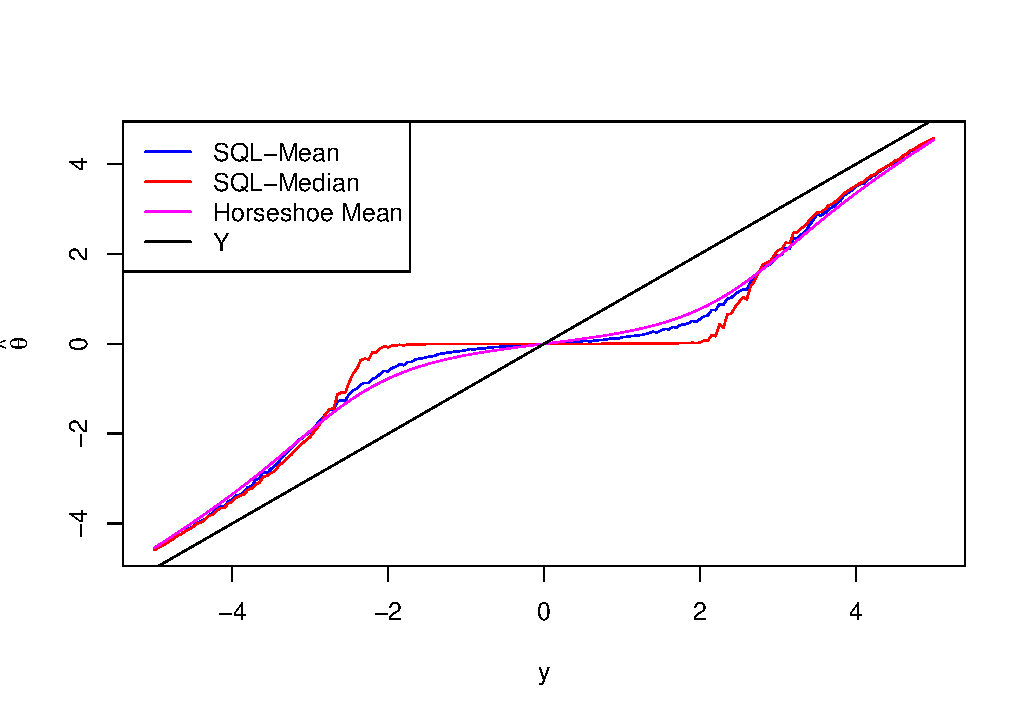
\includegraphics[width=0.7\columnwidth]{art/shrinkage_profile}%
\caption{Shrinkage profile for the horseshoe posterior mean and Bayesian \sql{} posterior mean and median estimators. }%
\label{fig:profile}%
	\end{figure}
\end{frame}

\begin{frame}
	\frametitle{Dependence on $\sigma^2$}
	\sql's main advantage is its ambivalence to the error variance $\sigma^2$. Does this property carry over to the Bayesian representation ?
	\heading{Horseshoe}
	Hierarchical model: 
\begin{align}
  (y_i \mid \beta_i) & \sim \Nor(\beta_i , \sigma^2), \;  (\beta_i \mid u_i, \tau) \sim 
  \Nor(0, u_i^2 \tau^2), \; u_i ^2 \sim \operatorname{C}^{+}(0,1).
  \label{eq:hs}
\end{align}

With different treatments available for $\tau.$ The following example from \cite{polson2010shrink} highlights the issue of dependence between $\tau$ and $\sigma^2$. 
\end{frame}

\begin{frame}
	\frametitle{Dependence on $\sigma^2$}
	%\cite{polson2010shrink} illustrate how Global-Local priors dependence on $\sigma^2$ might affect their performance. In Fig. \ref{fig:effect-sigma}, two observations were generated from $\NormRV(20,\sigma^2)$. The posterior distribution for different treatment of the parameter $\tau$.
	\begin{figure}%
\centering
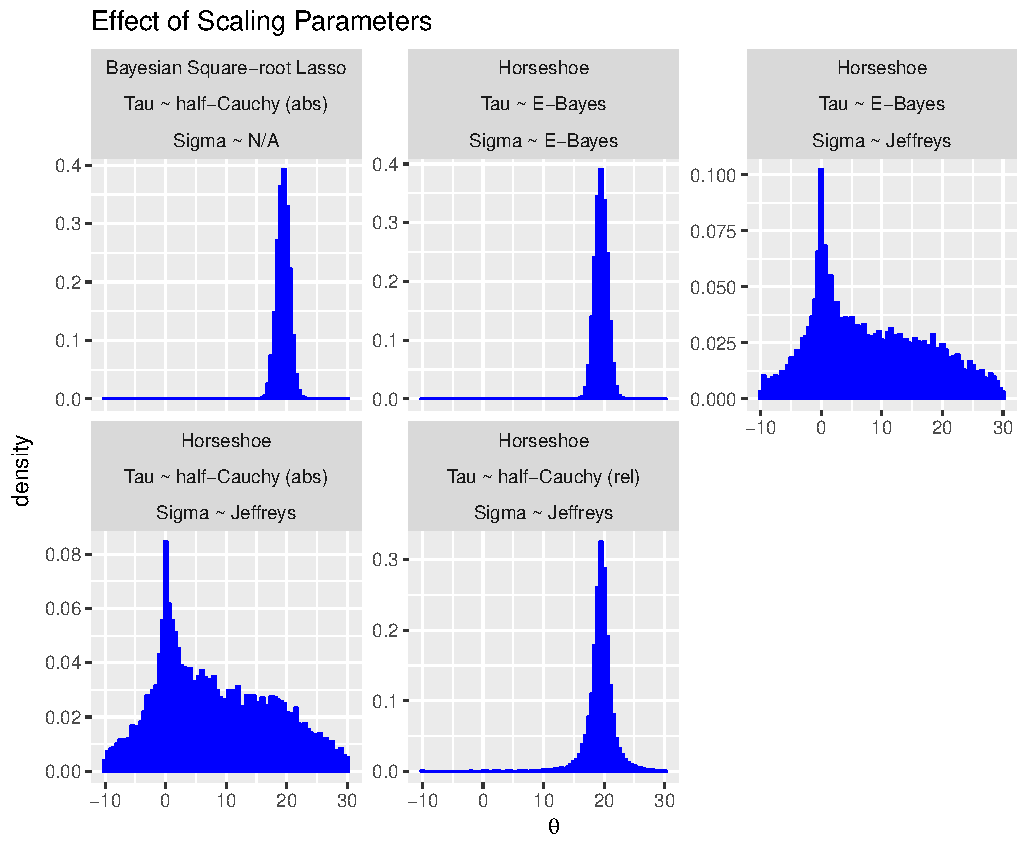
\includegraphics[width=0.75\columnwidth]{art/effect_of_sigma}%
\caption{Behavior of the posterior density under different methods of handling the hyper-parameters $\sigma^2$ and $\tau$ for the Horseshoe prior as well as the Bayesian \sql{}. }%
\label{fig:effect-sigma}%
	\end{figure}
\end{frame}

\section{Adding a Global Component}

\begin{frame}
	\frametitle{Global-Local Shrinkage priors}
	The prior placed on $\bbeta$ so far:\begin{equation} \label{Lasso_prior}
\beta_j \stackrel{iid}{\sim} \NormRV(0 , \tau_j^2), \ \tau_j^2  \stackrel{iid}{\sim} \mathcal{E}\mathrm{xp}(\lambda^2/2), \text{and } \lambda^2 \sim \pi \left(\lambda \right). 
\end{equation}
\begin{itemize}
	\item Independence of $(\beta_j \mid \lambda)$ $\Rightarrow$ inadequate prior mass on sparse regions.
	\item No global shrinkage parameter, that controls or accounts for sparsity.
\end{itemize}
\blankline
Instead G-L priors generally take the following form:\[ \beta_j \stackrel{iid}{\sim} \NormRV(0 , \tau^2 \psi_j^2), \ \psi_j \sim f \mbox{ and} \ \tau \sim g, \]
where:
\begin{itemize}
	\item $\tau$, controls how large the parameters are (like a penalty level);
	\item $\psi_j$, on the other hand  controls how big the parameter is allowed to be locally.
\end{itemize}
\end{frame}
\begin{frame}
	\frametitle{Dirichlet-Laplace prior}
	%\cite{bhattacharya2014dirichlet}, proposed a more intuitive parametrization, by constraining the $\psi_j$'s to a simplex. The idea is to model the joint distribution of the $\bbeta$ vector.
	%\heading{DL prior}
	Instead of a global parameter in \eqref{Lasso_prior}, \cite{bhattacharya2014dirichlet} introduced a vector of scales $\left( \phi_1 \tau , \ldots , \phi_p \tau \right)$, where $ \left( \phi_1 , \ldots , \phi_p \right) $ is constrained to lie in the $ (n - 1) $ dimensional simplex. 
	
	Their prior has the following form:
	$$ \beta_j \mid \phi , \tau \sim \text{\rm{DE}}(\phi_j \tau), \, \bphi \sim \text{\rm{Dir}}(a, \ldots ,a), \ \tau \sim g.$$ 
	
	This is the Dirichlet-Laplace prior on $\bbeta$, denoted as $\bbeta \mid \tau \sim \text{\rm{DL}}_a(\tau)$.
	\blankline
	
	
\begin{proposition}\label{DL_prior_carac}
If $\bbeta \mid \tau \sim \text{\rm{DL}}_a(\tau)$, then the marginal distribution of $\beta_j$ given $\tau$ is unbounded with a singularity at zero for any $a < 1$.
\end{proposition}
\end{frame}

\begin{frame}
	\frametitle{Tail and origin behavior}
	\begin{figure}%
	\centering
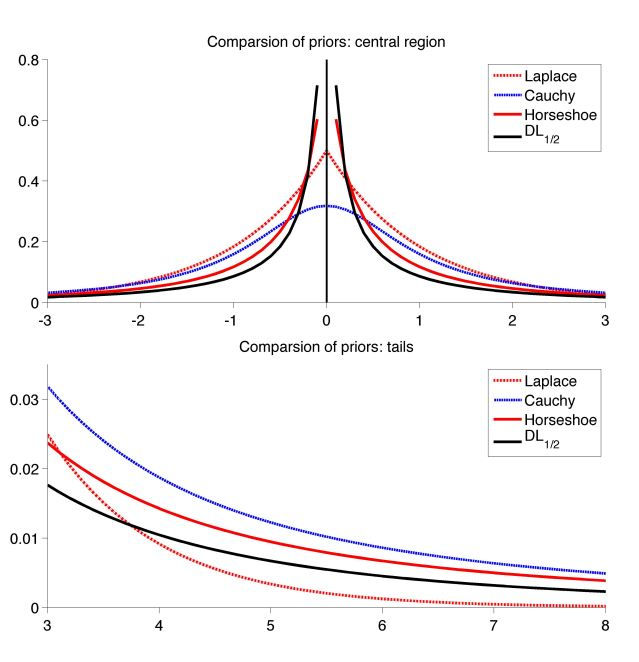
\includegraphics[width = .6\textwidth]{Priors}
\caption{Marginal density of the $\text{\rm{DL}}_a$ with $a = 1/2$ in comparison to the Horseshoe, the Laplace prior induced by the Bayesian-$\sqrt{\text{Lasso}}$ and the Cauchy prior.}
\label{fig_priors}
	\end{figure}
\end{frame}

\begin{frame}
	\frametitle{Hierarchical Model}
	Again using the scale mixture representation of the Laplace distribution:\[ \beta_j \mid \phi , \tau \sim \text{\rm{DE}}(\phi_j \tau) \Rightarrow \left\{ \begin{array}{ccc}
\beta_j & \sim & \NormRV(0 , \psi_j\phi^2_j\tau^2); \\
\psi & \sim & \mathcal{E}\mathrm{xp}(1/2),
\end{array} \right. \] we get the following full hierarchical model:
\begin{align*} \label{sq_dl_h}
[ \y \mid \bbeta, v^2 ] & \sim \NormRV(\X \bbeta, v^2 \I_n), \\
[\bbeta \mid \bphi, \tau , \bpsi ]  &\sim \NormRV(\0, D_{\bpsi \bphi \tau}), \\ D_{\bpsi \bphi \tau} &= \text{Diag}(\psi\phi_1^2\tau^2, \ldots, \psi\phi_p^2\tau^2), \\
\psi_j & \stackrel{iid}{\sim} \mathcal{E}\mathrm{xp}(1/2), \\
\bphi & \sim \text{\rm{Dir}}(a, \ldots ,a), \\
\frac{\tau}{v^2}  &\sim \mathcal{G}\mathrm{amma}(pa , 1/2), \\ 
[v^2] &\sim \mathcal{G}\mathrm{amma}(\frac{n+1}{2} , 1/2).  
%[\tau^2] & \sim p(\tau^2) d\tau^2,  \; \tau^2 > 0. \quad [ \tau^2 \sim \GammaRV(r, \delta), \text{ or } \tau^2 \sim \CauchyRV(0,1). ]
\end{align*}
\end{frame}

\begin{frame}
	\frametitle{Posterior Computation}
	Full conditionals for the Gibbs sampler:
	\begin{itemize}
\item[(i)] Sample $[ \bbeta \mid \bpsi , \bphi , \tau , \v^2 , \y ]$ from $\NormRV \left( \bSigma \X^T\y/v^2 , \bSigma \right)$, with $$ \bSigma^{-1} = \frac{\X\X^T}{v^2} + \frac{\D^{-1}_{\bpsi \bphi^2}}{\tau^2}.$$
\item[(ii)]Conditional posterior of $[\bpsi \mid \bphi , \tau , \bbeta]$ can sampled in block  by independently drawing $ \psi_j \mid \phi_j , \tau , \beta_j $ from 
$ \text{inv-Gaussian}(\frac{\phi_j\tau}{\abs{\beta_j}} ,1) $
\item[(iii)] Sample the conditional posterior of $[ \bphi \mid \bbeta]$ by drawing $ \ T_1, \ldots \T_p$ independently from $\text{gIG}(a-1 , 1 , 2\abs{\beta_j})$ and set $\phi_j = T_j/T$, with $T = \sum_{j=1}^{p}T_j$.
\item[(iv)] Sample $[ \tau \mid \bphi, \bbeta, v^2 ]$ from a $\text{gIG}( pa-p , 1 , 2\sum^{p}_{j=1}\abs{\beta_j}/\phi_j )$ distribution.
\item[(v)] Sample $[ v^2 \mid \bbeta ,\tau , \y ]  $ by drawing $ \frac{1}{\sigma^2} $ from $\text{inv-Gaussian}( [ \norm{\y - \X\bbeta} + \tau ]^{-1} ,1) $.
\end{itemize}
	
\end{frame}

%\section{Computational Issues}


\section{Simulations}

\begin{frame}
	\frametitle{Sparse Normal Means}
	In the normal means problem, the goal is to estimate a sparse vector $\btheta$ based on a vector $\Y = \left(Y_1, \ldots , Y_n \right) $ generated according to the model:
\begin{equation}\label{normal_means}
Y_i = \theta_i + \epsilon_i, \quad i = 1, \ldots, n.
\end{equation}
where $\epsilon_i$'s are independent standard normal variables and the means vector $\btheta$ is assumed to be sparse.

We conduct a simulation study for estimating a sparse normal mean vector for two different choices of $\bbeta$: 
\blankline
\ben
\item $\bbeta = (\underbrace{7,\ldots,7}_{q_n=10},\overbrace{0,\ldots,0}^{n-q_n = 90})$ and 
\item $\bbeta = (\underbrace{7,\ldots,7}_{q_{n}=10},\underbrace{3,\ldots,3}_{r_n=10}\overbrace{0,\ldots,0}^{n-q_n-r_n = 80})$.
\een
%We generate observations from a Gaussian model $(y_i \mid \beta_i) \sim \NormRV(\beta_i, \sigma^2)$ for $\sigma^2 = 1$ and $\sigma^2 = \half$.
\end{frame}

\begin{frame}
	%\frametitle{Sparse Normal Means}
	\begin{figure}[!ht]%
\centering
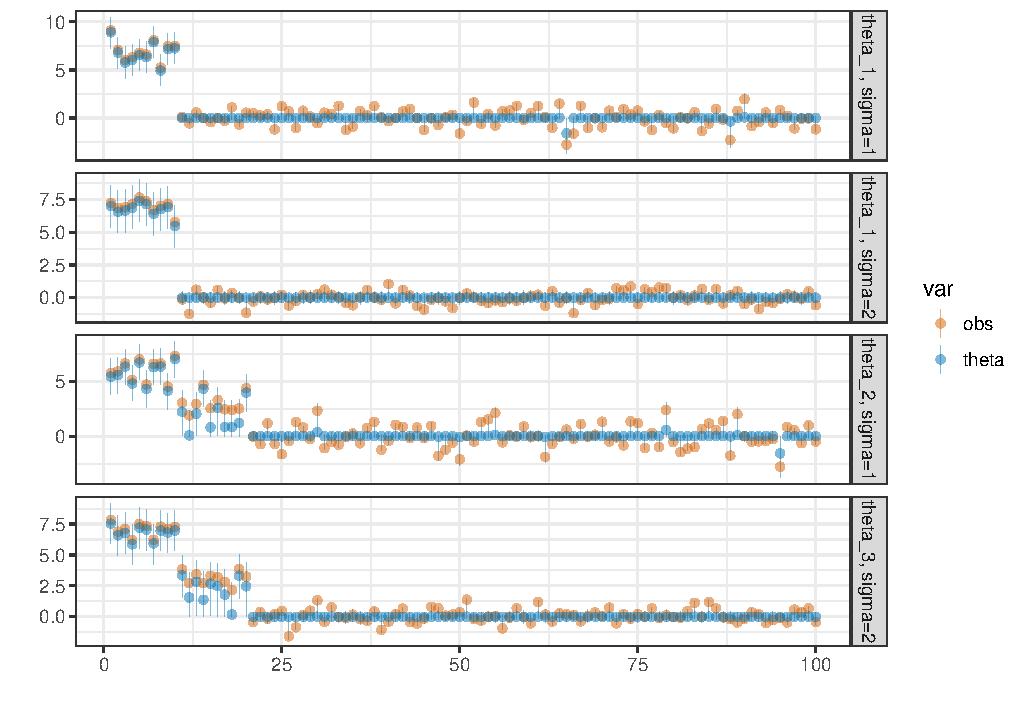
\includegraphics[width=\columnwidth]{art/sparse-means-sql-1}%
\caption{Comparison of posterior mean estimates for two different sparse normal means, $\beta_i \sim 0.8 \delta_{\{7\}}+0.1\delta_{\{3\}}+0.1\delta_{\{0\}}$ and $\beta_i \sim 0.9 \delta_{\{7\}}+0.1\delta_{\{0\}}$ under the Bayesian $\sqrt{\text{Lasso}}$ . }%
\label{fig:sql-sim-1}%
\end{figure}
\end{frame}

\begin{frame}
	\frametitle{Regression and Variable Selection}
	Another important area of application of shrinkage priors, is regression and particularly model selection:
$$ \y  = \X\bbeta + \bepsilon, \quad \text{with } \bepsilon \sim \NormRV(\0 , \sigma^2 \I_n ) $$
where $\bbeta$ is $p\times 1$ and is assumed to be sparse. Sparsity implies that some of the regression coefficients are exactly zero and they correspond to irrelevant predictors. 

Motivated by the two groups model \eqref{eq:2groups} and the necessity of a variable selection step for the Bayesian methods, we apply a 2-means clustering of the posterior estimates.
\beq \label{eq:2groups}
\beta_i \sim \tfrac{q}{p} \delta_{A} + \tfrac{p-q}{p} \delta_{0}, \ \text{so that }  \bbeta = ( \underbrace{ A, \ldots ,A}_{q}, \overbrace{0, \ldots 0}^{p-q} )
\eeq

\end{frame}

\begin{frame}
	\frametitle{Regression and Variable Selection}
	After clustering the posterior mean vector, we classify the $\beta$'s according to the following steps : 
	
\ben
\item[1-] We look first at the two cluster centers $\left\lbrace \c_1 , \c_2 \right\rbrace $, and compare them in absolute value. Let $\C_s = max\left\lbrace \c_1 , \c_2 \right\rbrace$ and $\c_n = min\left\lbrace \c_1 , \c_2 \right\rbrace$. So that the $\c_s$ is the cluster center of the signals while $\c_n$ for the noise.
\item[2-] For all $\hat{\beta_j}$, look at the corresponding cluster, if $\abs{\hat{\beta_j}} \in \c_n $, then $\hat{\beta}_j^{dec}= 0$. Otherwise, $\hat{\beta}_j^{dec} = \hat{\beta_j}$.
\item[3-] Our final estimated coefficient vector is $\hat{\bbeta}^{dec} = \left\lbrace \hat{\beta}^{dec}_{j} \right\rbrace_{1\leq j \leq p}$.
\een

Unlike $\hat{\bbeta}$, which will never have exactly zero entries, the new $\hat{\bbeta}^{dec}$ given by the above described decision rule shrinks the noise coefficients to exactly zero, hence performing a variable selection.
\end{frame}

\begin{frame}
	\frametitle{Consistency}
	%One of the many interesting questions that arise with variable selection, is \textit{Model selection consistency}. This property essentially means that the method used consistently selects the true model. It should be emphasized that model selection consistency and estimator consistency are entirely two different properties. 
	Estimation consistency holds if and only if:\[ \hat{\bbeta}^{n} -  \bbeta \stackrel{\P}{\longrightarrow}0, \ \text{as } n\longrightarrow \infty,  \]
while model selection consistency requires:
\[ \P\left[ \lbrace i : \hat{\beta}_i^{n} \neq 0 \rbrace = \lbrace i : \beta_i \neq 0\rbrace \right] \longrightarrow 1, \ \text{as } n\longrightarrow \infty. \]
%Some authors have also considered sign consistency. 
Characterizing a method model selection performance has proven to be a daunting task. However, in the case of the Lasso, some authors have found that there a exist one simple necessary and sufficient condition for the Lasso to select the true model.

\end{frame}

\begin{frame}
	\frametitle{Irrepresentability Condition}
	Suppose, the sample covariance matrix is denoted by $\hat{\Sigma} = nX^T X$ and the active-set $S_0 = \{ j : \beta_j \neq 0\}$ consists of first $s_0$ elements of $\beta$. One can partition the $\hat{\Sigma}$ matrix as
$$ \hat{\Sigma} = \left(\begin{array}{cc}
\hat{\Sigma}{s_0,s_0} & \hat{\Sigma}{s_0,p-s_0} \\ \hat{\Sigma}{p-s_0,s_0} & \hat{\Sigma}{p-s_0,p-s_0} \end{array} \right) $$
 The irrepresentable condition for variable selection consistency of Lasso is:
$$ || \hat{\Sigma}{p-s_0,s_0} \hat{\Sigma}{s_0,s_0}^{-1} sign(\beta_{S_0}) ||_{\infty} \leq \theta \quad \mbox{ for some } 0 < \theta < 1 .$$

Zhao et al.[2006], this condition is sufficient and almost necessary.

They also showed that the probability of selecting the true sparse model is an increasing function of the irrepresentability condition number, defined as $$ \eta_{\infty} = 1 - || \hat{\Sigma}{p-s_0,s_0} \hat{\Sigma}{s_0,s_0}^{-1} sign(\beta_{S_0}) ||_{\infty} . $$
\end{frame}

\begin{frame}
	\frametitle{Effect of irrepresentability}
	\bit 
	\item Simulation scheme: $n = 100, p = 60$ and $q = 7$, $\beta_{q}^* = (7,5,5,4,4,3,3)^T$, $\sigma^2$ was set to $5$ to allow for heavy tailed data. 
	\item First draw $\Sigma$ from $\text{Wishart}(p, I_p)$ and then generate $\X$ from $\Nor(0,\Sigma)$ \citep{zhao2006model}.
	\item Generate $100$ different design matrices, and run $100$ replicates of each one, and at each iteration we apply the Lasso, horseshoe, Bayesian-$\sqrt{\text{Lasso}}$ and the $\sqrt{\text{\rm{DL}}}$ 100 times to each of the $100$ generated models. 
	\item Select the posterior median and then apply a variable selection step. \textcolor[rgb]{0.5,0,0.5}{For the horseshoe, we take advantage of the credible set properties and use them to classify the $\beta_j$'s. For the other two methods discussed in this work, we implement the k-means clustering procedure discussed previously.}
	\eit
\end{frame}

\begin{frame}
	\frametitle{Results}
	\begin{figure}
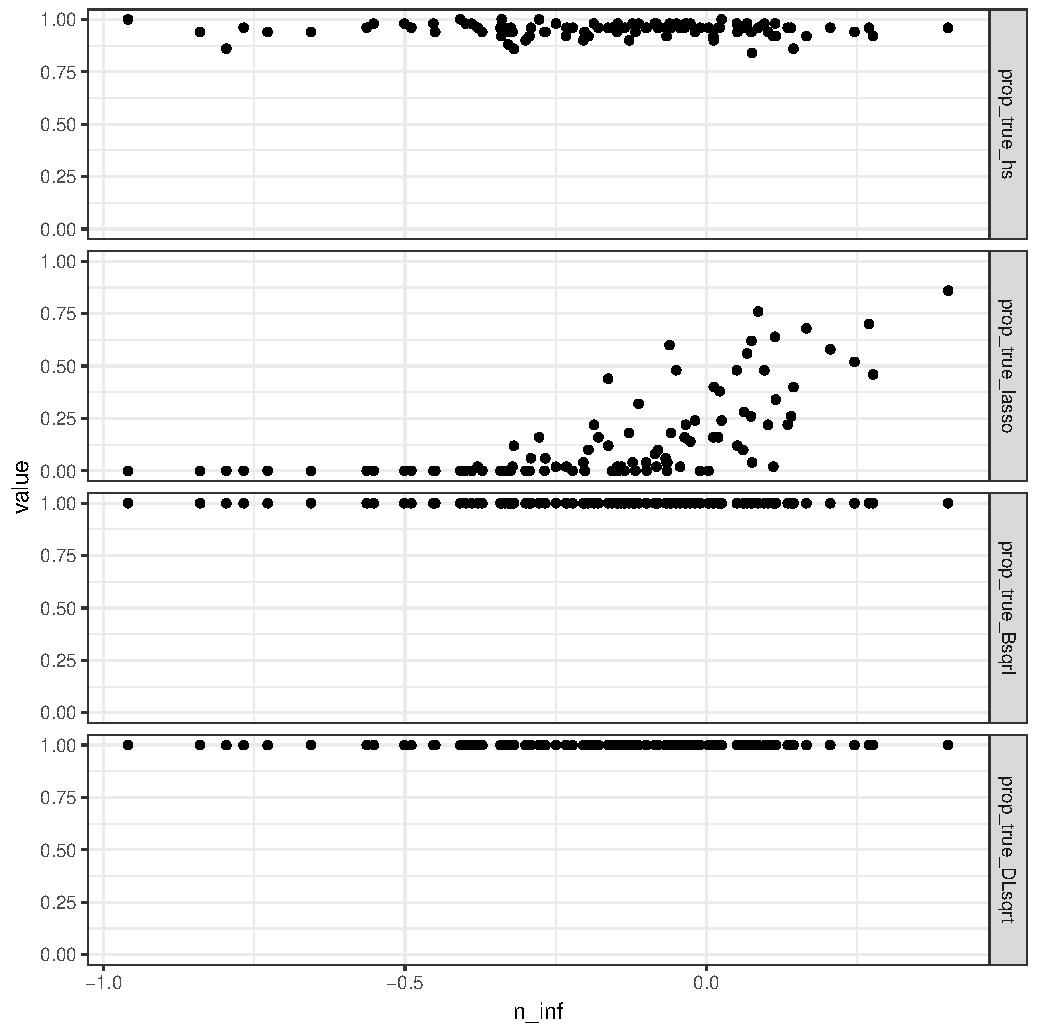
\includegraphics[width=0.75\columnwidth , height =.8\textheight]{Irrep_model_selec_n100p60_q50_2groups}%
\caption{Proportion of true model selection vs. Irrepresentability Condition}%
\label{fig:profile:MSP_irrep}%
\end{figure}
\end{frame}
\begin{frame}
	\frametitle{Results}
	\begin{figure}
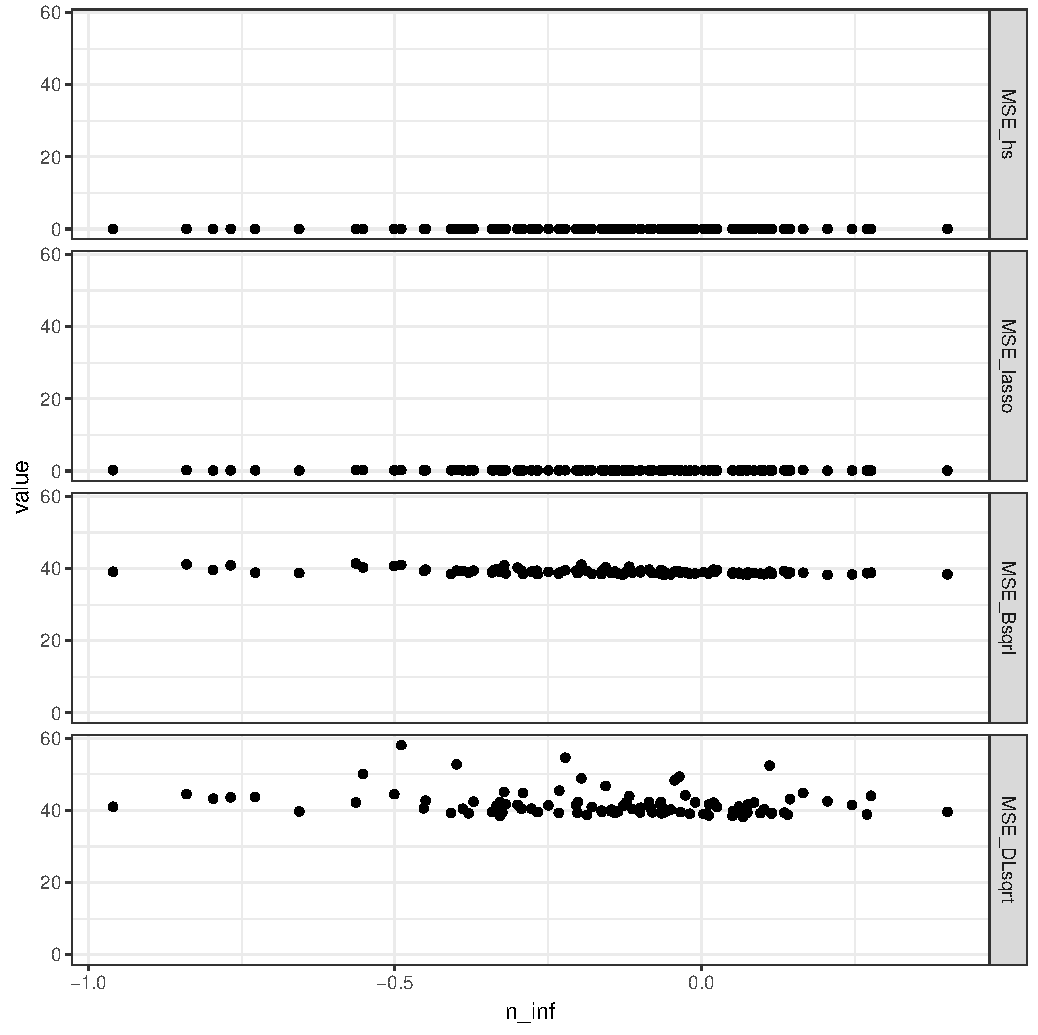
\includegraphics[width=0.75\columnwidth , height =.8\textheight]{Irrep_MSE_selec_n100p60_q50_2groups}%
\caption{MSE vs. Irrepresentability Condition }%
\label{fig:profile:MSP_irrep}%
\end{figure}
\end{frame}

\begin{frame}
	\frametitle{Adapting to Sparsity ?}
	\bit
	\item Most penalized regression methods, and shrinkage priors operate under the assumption that the parameter of interest is sparse.	
	\item \textbf{What if $\bbeta_0$ has zero entries but is not completely sparse ?} 
	%Here we try to address this issue by running simulations on model designs with varying underlying levels of sparsity.
	
	\item Simulated data with $n = p = 100$, the design matrix $\X$ rows were simulated from a univariate normal distribution $\NormRV(0 ,2)$, the errors variance was set to $\bsigma^2 = 5 $. 
	
	\item Sampled $100$ different design matrices, and for each of these design matrices, applied the four different methods with varying degrees of sparsity. That is for each of the $100$ designs, say $\X$, we have nine different response vectors obeying the following equation:
$$
\y^{k} = \X \bbeta^{k} + \bepsilon, \ \text{where } \bbeta^{k} =  ( \underbrace{ 5, \ldots ,5}_{q = k\nicefrac{p}{10}}, \overbrace{0, \ldots 0}^{p-q} ) \ \text{for } k = 1,\ldots, 9 .
$$
\eit
%Hence for each sparsity level, we have a $100$ replicates, from which we compute the misclassification proportion, that is the number of times a given method does not select the true model, and the MSE. Here we also compute for the Bayesian methods, the MSE after the decision rule was performed $\textbf{\rm{MSE}}(\hat{\bbeta}^{dec})$. 
\end{frame}

\begin{frame}{Effect of Sparsity}
	%\frametitle{Misclassification proportion}
	\begin{figure}
\centering
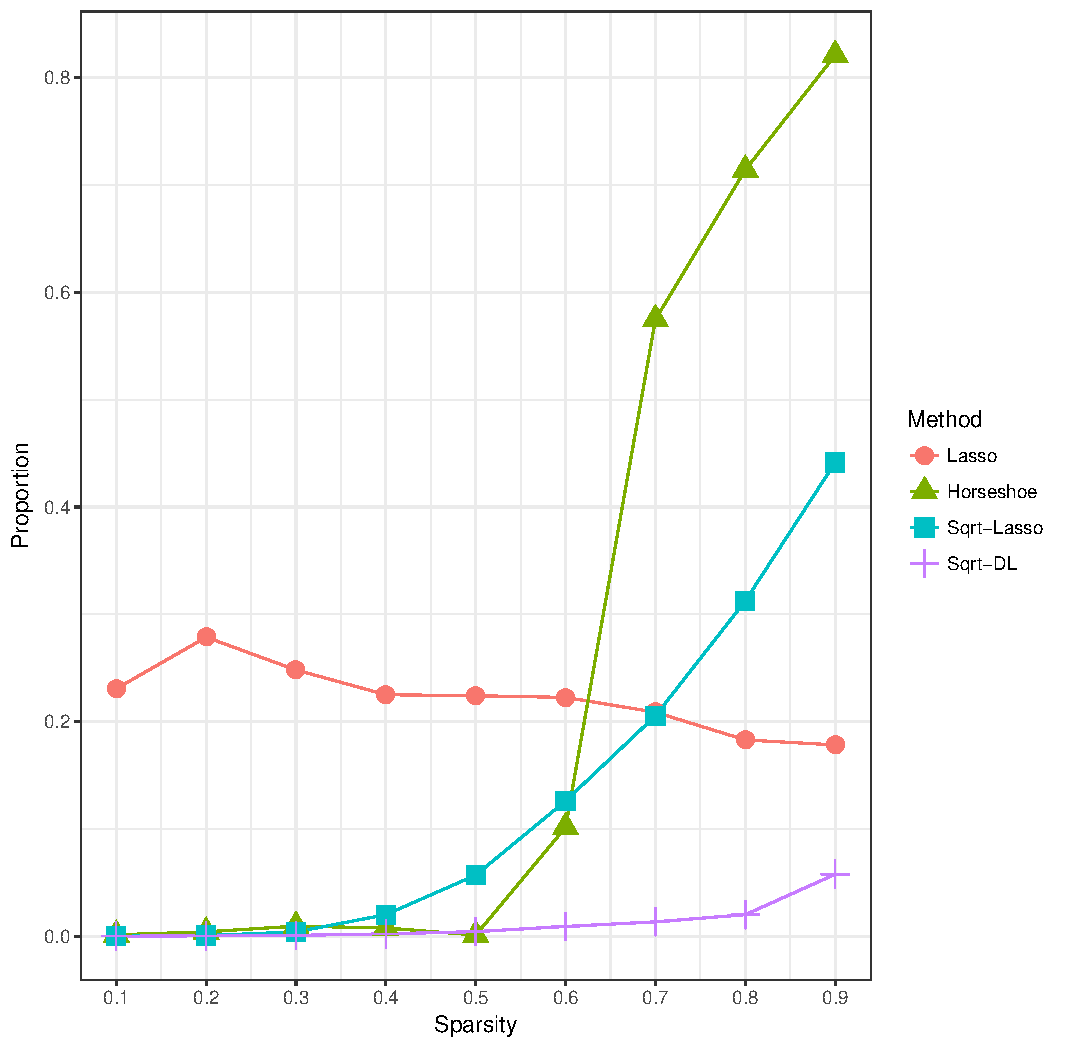
\includegraphics[height = .85\textheight , width = \linewidth]{Sparsity_MSP_n=p}
\caption{Misclassification proportion as a function of sparsity level.}
\label{fig:msp}
\end{figure}
\end{frame}

\begin{frame}{MSE as a function of sparsity}
	%\frametitle{}
	\begin{figure}[h!]
  \centering
  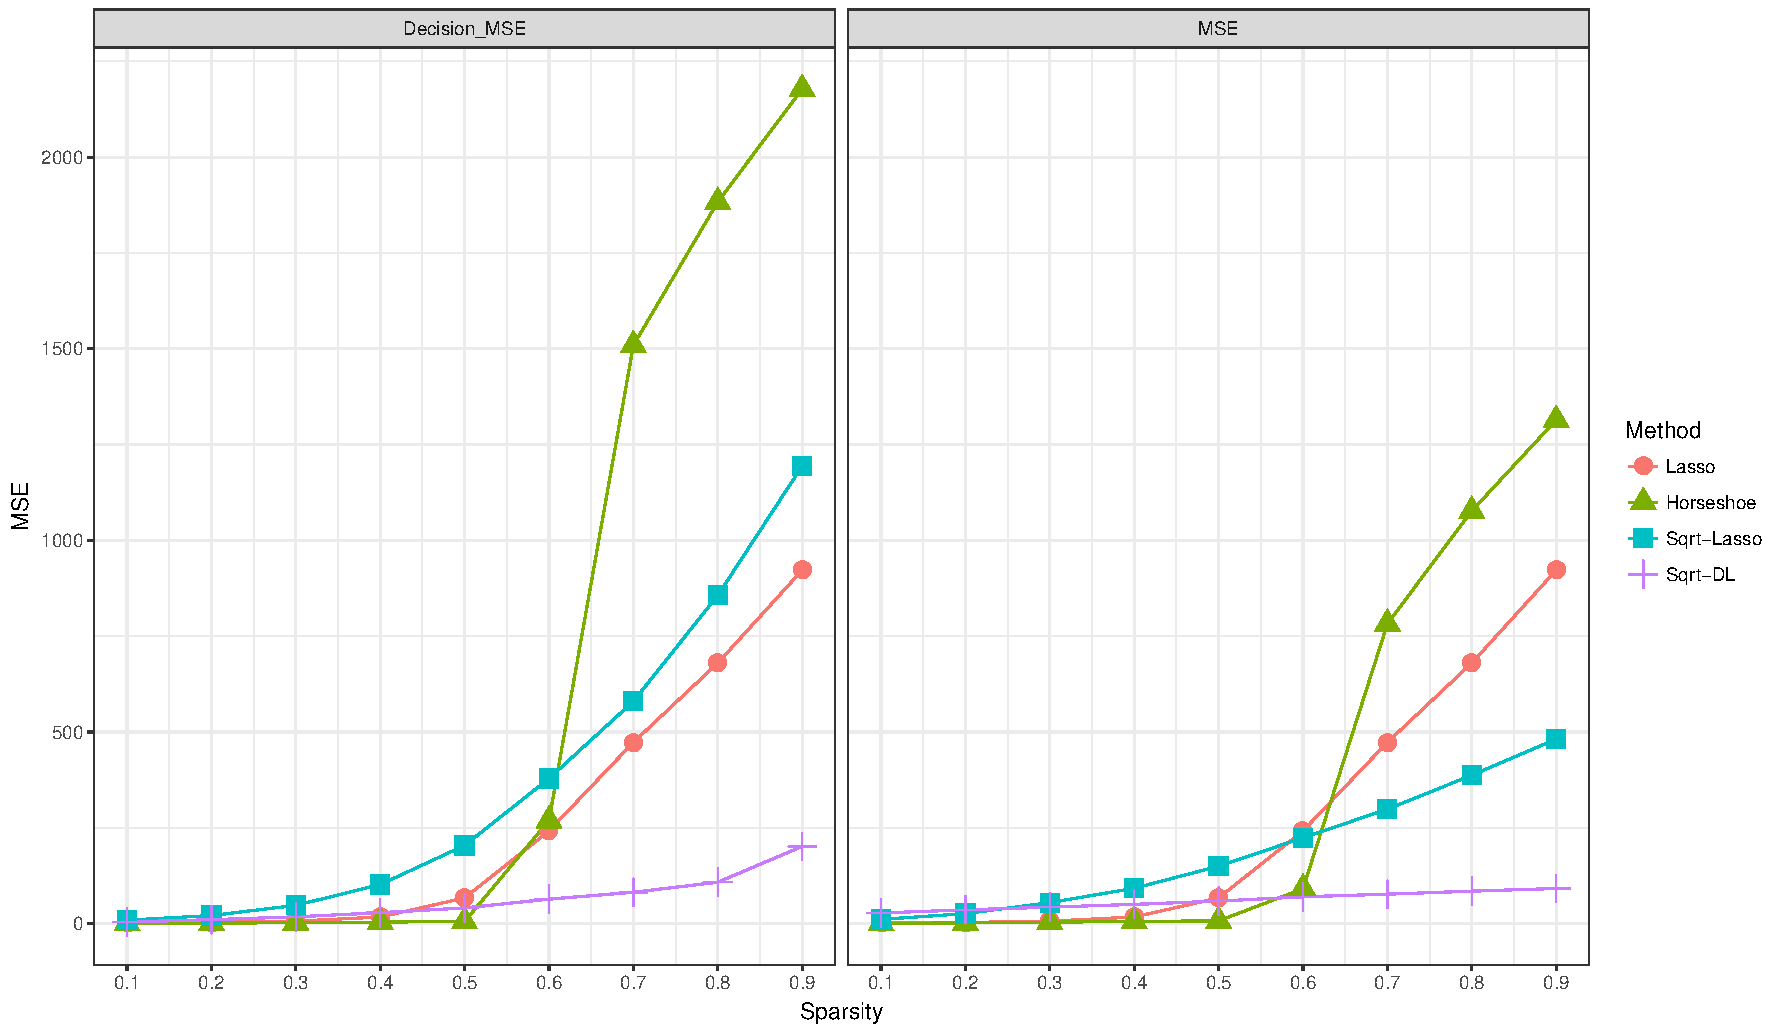
\includegraphics[width=\linewidth , height = .85\textheight ]{Sparsity_MSE_high_n=p}\caption{A comparison of the MSE as a function of sparsity level}
\label{fig:test}
\end{figure}
\end{frame}


\section{Discussion}
\begin{frame}
\frametitle{Discussion}
In this work, we first developed:

\begin{itemize}
	\item  a Bayesian representation of the \sql;
	\item using normal scale mixtures we developed a corresponding Gibbs sampler;
	\item unlike the horseshoe and G-L shrinkage priors, this method obviates the need to learn, scale or estimate the precision parameter $\sigma$;
	\item motivated by the strong properties G-L priors, added a global component to our model. This ensured, that the new prior placed sufficient mass around the origin, thus a priori favoring nearly black sets; 
	\item yet we did not observe any improvement in concentration coverage, as the MSE stayed quite high in our empirical investigation.
	\end{itemize}
		
		\blankline
		 Surprisingly, the effect of the added global parameter was a nice adaptability to sparsity levels. This new interesting property requires more theoretical investigation. 

 
%\item Theoretical Justification for sparsity and dependence
 %In Fig. \ref{fig:tau-hs}, we see how in the case of the horseshoe the boxplots for the $\btau$ samples continue to increase until we reach  level of approximately $.5$ where a dramatic breakdown happens. Clearly, in the left side of the figure, we can say that $\btau$ follows the monotone increase in the proportion of non-zero parameters, but when this proportion approaches and exceeds the $.5$ threshold, the method is no longer able to follow and adapt the sparsity level. This behavior also explains why the MSE and the proportion of misclassified $\beta$'s exploded whenever the proportion of non-zero $\beta$'s exceeded the threshold of $0.5$, as shown in Fig \ref{fig:msp} and Fig. \ref{fig:test}.


%On the other hand, we also saw in Fig \ref{fig:msp} and Fig. \ref{fig:test}, how the \sqdl performance remained satisfactory and was in no way affected by changes in the sparsity level. The boxplots of $\btau$ samples in Fig. \ref{fig:tau-dl}, back up our conjecture, unlike the horseshoe, here the global shrinkage parameter follows and learns correctly the degree of sparsity. In the future, we would like to theoretically investigate this claim and try to prove it.




%item extension to non gaussian likelihood \cite{datta2016bayesian}


\end{frame}

\begin{frame}
\frametitle{Effect of Sparsity on $\tau$}
We conducted a small experiment, where models with different proportions of non-zero parameters were constructed, and we implemented both the \sqdl and the horseshoe.
\begin{figure}
\centering
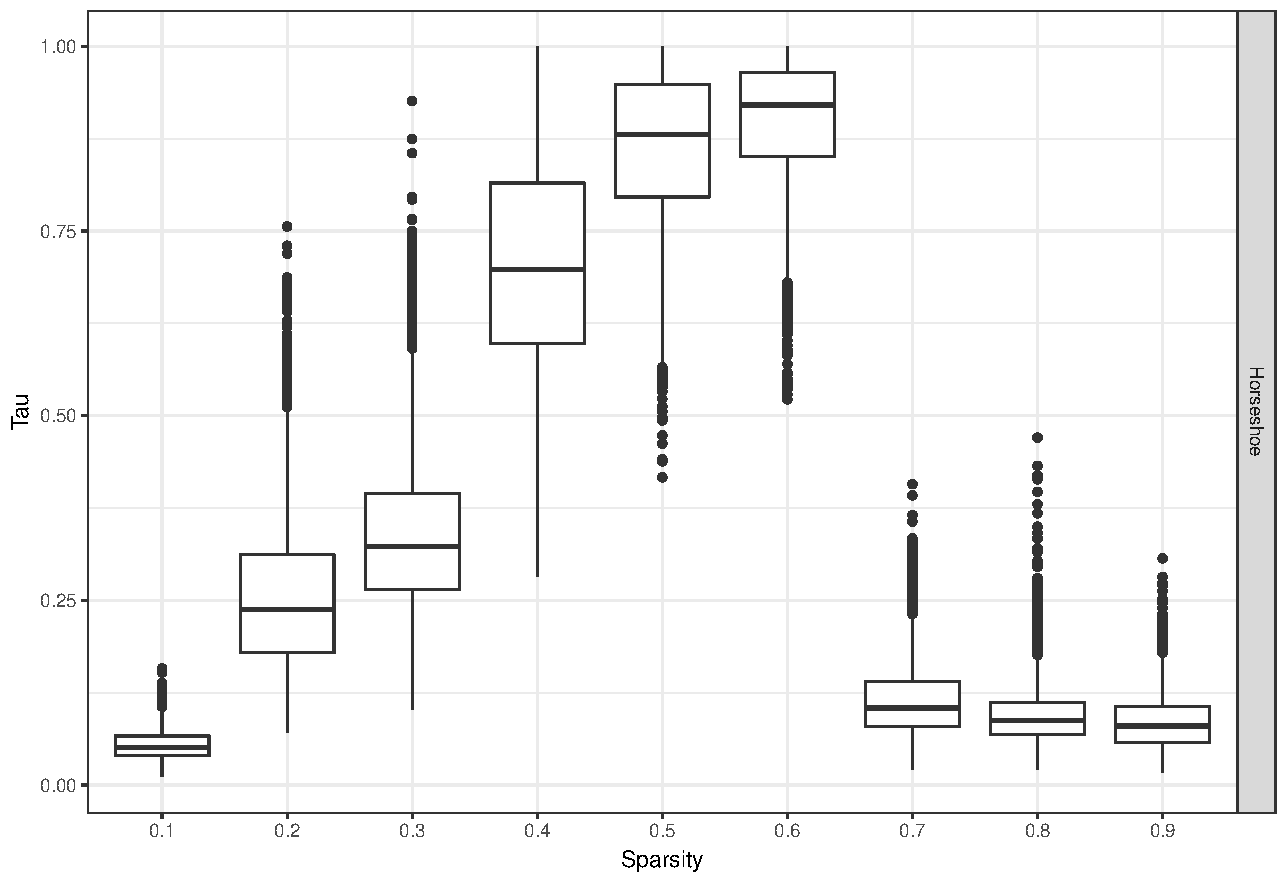
\includegraphics[width = .9\columnwidth , height = .7\textheight]{Tau_hs}\caption{Evolution of $\btau$ in terms of sparsity level for the Horseshoe method}\label{fig:tau-hs}
\end{figure}
\end{frame}

\begin{frame}
\frametitle{Effect of Sparsity on $\tau$}
\begin{figure}
\centering
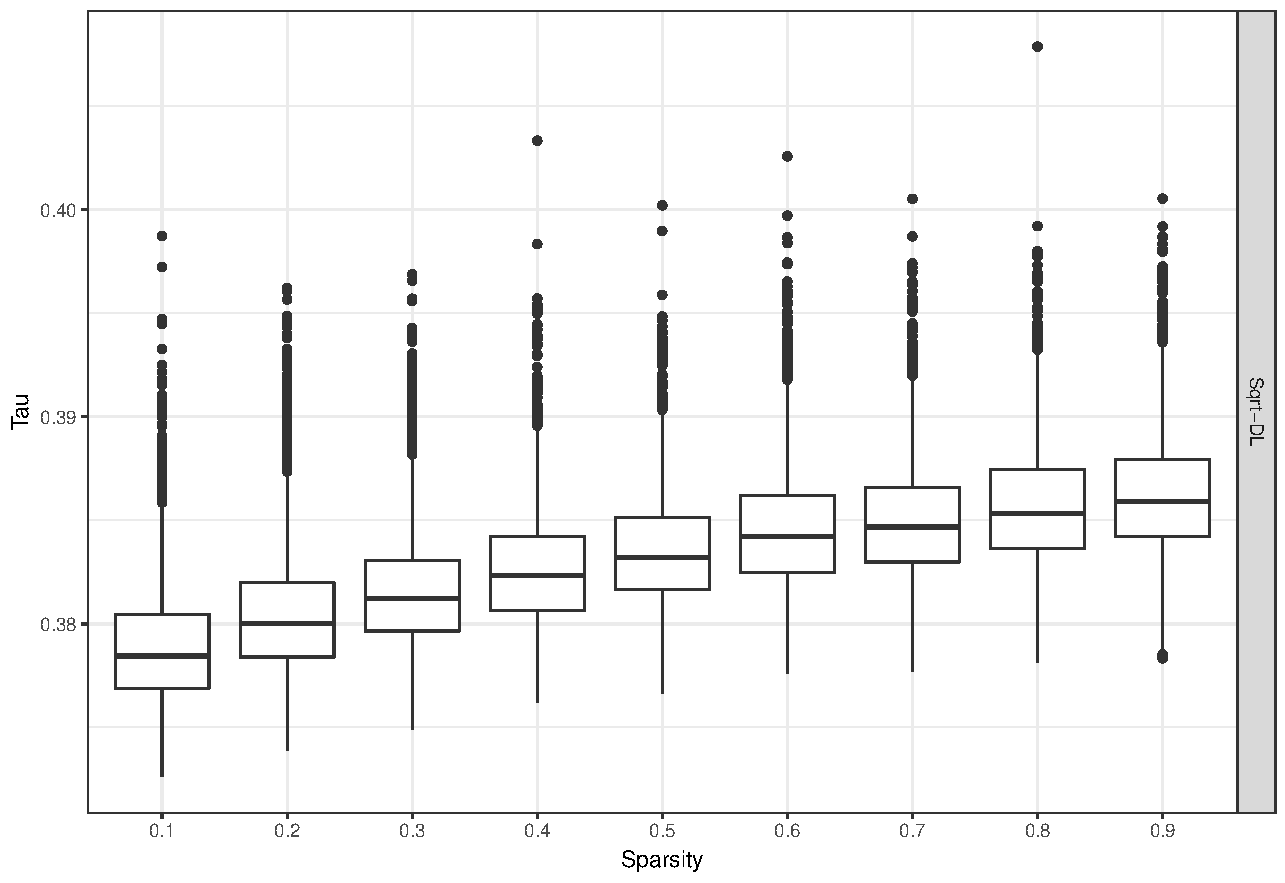
\includegraphics[width = .9\columnwidth , height = .7\textheight]{Tau_dl}\caption{Evolution of $\btau$ in terms of sparsity level for the \sqdl method}\label{fig:tau-dl}
\end{figure}
\end{frame}

\begin{frame}{Computational Concerns}
\begin{itemize}
	\item Handling global parameters: full Bayes / MMLE / CV / $m_{eff}$.
	\item Gometric convergence of MCMC is not guaranteed.
	\item Rao-Blackwellization of global parameters.
\end{itemize}
	
\end{frame}

\begin{frame}
\frametitle{Future Directions}
\begin{itemize}
	\item Theoretically investigate and prove adaptability to sparsity of \sqdl;
	\item Extend the methods developed here to the case of non-gaussian likelihood, such as count and categorical data.
	\item The Bayesian \sql{} and \sqdl will be investigated \textit{vis-a-vis} other G-L priors tailored for Gaussian data when the error distribution is heavy-tailed, e.g. $t$-distribution.
\end{itemize}
\end{frame}

\begin{frame}{}
\heading{Thanks!!}
\end{frame}
\bibliographystyle{plainnat}
%\nobibliography{rsref,citation,horseshoe-plus}
\nobibliography{sqlassorefs,hs-review}
\end{document}
